\section{Introduction.}
%
\begin{print}
 The CFS project was developed for solution of partial differential equations by means of finite element as well as boundary element method. It was projected, keeping in mind to use it for the implementation of adaptivity for FE/BE methods. Another important criteria for design of this code is ability to solve coupled field problems. Code of CFS was implemented on C++ programming languages due to object-oriented concept of it. Hierarchy of classes, virtual classes, mechanizmes of templates play an important role throughtout implementation. For the code development we used GNU C++ compiler( version 2.95)  on LINUX and CC on SGI. At present scalar problem such as acoustic equation can be treated, It is solved by using the Newmark method.\\
 We give a sketch of design of programm and some issues of implementation. 
\end{print}
%
\newslide
%
\section{ Design criteria .}
\begin{itemize}
%
\item{\em separation of topological and algebraic entities}\\
%
\begin{print}
 It is an important criteria for design of code for implementation of adaptivity due to complexity of work with grid. By using global node-numbering strategy we are able to transfer structure of grid into algebraic structure.
\end{print}
%
\item{\em clear structure of code}\\
\begin{print}
 It should be easy to catch the structure of the program for users to be able to implement its own practical problems. So it should be designed in the way to hide and shield some structures and data from users.
\end{print}
%
\item{\em efficiency}\\
\begin{print}
 At the same time it should be efficient, because computations are often time-consuming, especially in 3D. Of course, this and former criteria are contracdictory and each time we have to trade against each other.
\end{print}
%
\item{ \em features of coupled field problems }\\
\begin{print}
 One of the main goal is to provide a program for the general handling of coupled field problems. Therewith, matrix as well as right hand side coupling will be supported.  
\end{print}
\end{itemize}
%
\newslide
%
\section{ Structure of code.}
\begin{figure}[H]
\begin{center}
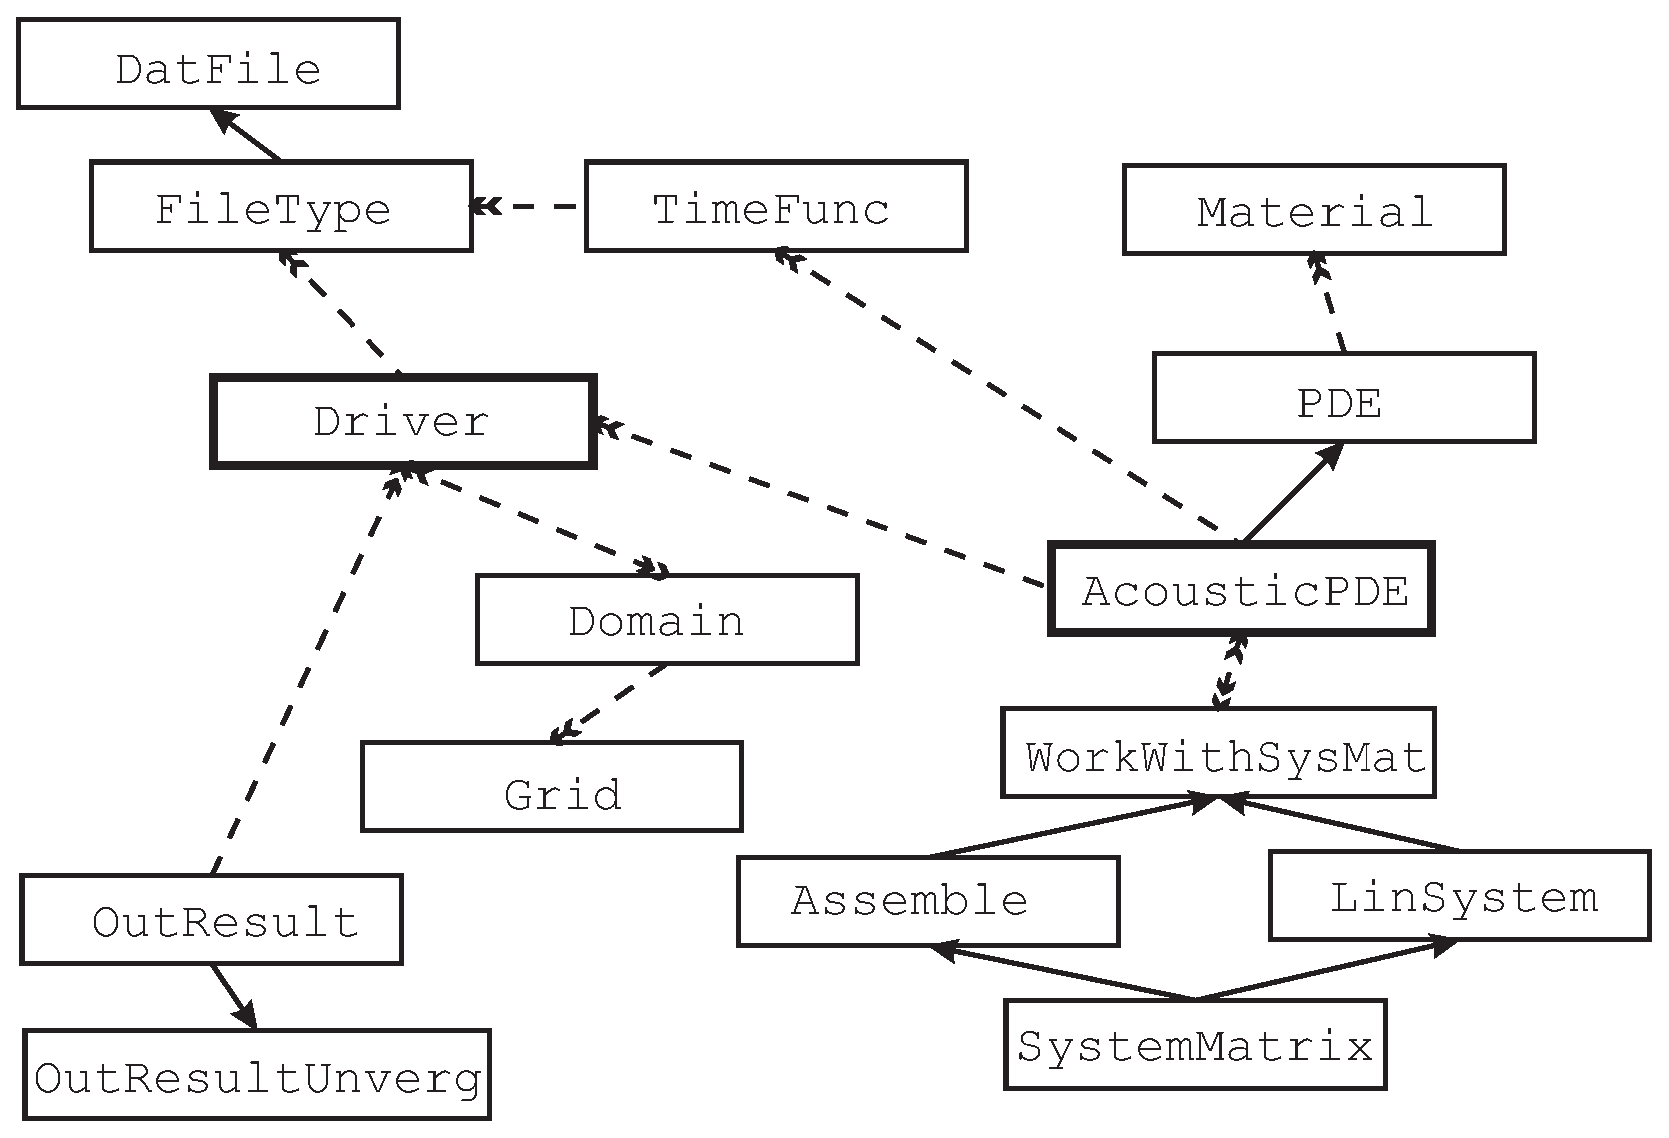
\includegraphics [width=8cm, angle=0] {./pic/main1}
\end{center}
\caption{ Structure of CFS }  
\end{figure}
\newslide
\begin{print}
 The main classes of code are shown on the figure. We give a short description of
these classes.
\end{print}
\newslide
